% Options for packages loaded elsewhere
\PassOptionsToPackage{unicode}{hyperref}
\PassOptionsToPackage{hyphens}{url}
\PassOptionsToPackage{dvipsnames,svgnames,x11names}{xcolor}
%
\documentclass[
  12pt,
  a4paper,
]{article}
\usepackage{amsmath,amssymb}
\usepackage{lmodern}
\usepackage{iftex}
\ifPDFTeX
  \usepackage[T1]{fontenc}
  \usepackage[utf8]{inputenc}
  \usepackage{textcomp} % provide euro and other symbols
\else % if luatex or xetex
  \usepackage{unicode-math}
  \defaultfontfeatures{Scale=MatchLowercase}
  \defaultfontfeatures[\rmfamily]{Ligatures=TeX,Scale=1}
\fi
% Use upquote if available, for straight quotes in verbatim environments
\IfFileExists{upquote.sty}{\usepackage{upquote}}{}
\IfFileExists{microtype.sty}{% use microtype if available
  \usepackage[]{microtype}
  \UseMicrotypeSet[protrusion]{basicmath} % disable protrusion for tt fonts
}{}
\makeatletter
\@ifundefined{KOMAClassName}{% if non-KOMA class
  \IfFileExists{parskip.sty}{%
    \usepackage{parskip}
  }{% else
    \setlength{\parindent}{0pt}
    \setlength{\parskip}{6pt plus 2pt minus 1pt}}
}{% if KOMA class
  \KOMAoptions{parskip=half}}
\makeatother
\usepackage{xcolor}
\IfFileExists{xurl.sty}{\usepackage{xurl}}{} % add URL line breaks if available
\IfFileExists{bookmark.sty}{\usepackage{bookmark}}{\usepackage{hyperref}}
\hypersetup{
  colorlinks=true,
  linkcolor={Maroon},
  filecolor={Maroon},
  citecolor={Blue},
  urlcolor={Blue},
  pdfcreator={LaTeX via pandoc}}
\urlstyle{same} % disable monospaced font for URLs
\usepackage{color}
\usepackage{fancyvrb}
\newcommand{\VerbBar}{|}
\newcommand{\VERB}{\Verb[commandchars=\\\{\}]}
\DefineVerbatimEnvironment{Highlighting}{Verbatim}{commandchars=\\\{\}}
% Add ',fontsize=\small' for more characters per line
\newenvironment{Shaded}{}{}
\newcommand{\AlertTok}[1]{\textcolor[rgb]{1.00,0.00,0.00}{\textbf{#1}}}
\newcommand{\AnnotationTok}[1]{\textcolor[rgb]{0.38,0.63,0.69}{\textbf{\textit{#1}}}}
\newcommand{\AttributeTok}[1]{\textcolor[rgb]{0.49,0.56,0.16}{#1}}
\newcommand{\BaseNTok}[1]{\textcolor[rgb]{0.25,0.63,0.44}{#1}}
\newcommand{\BuiltInTok}[1]{#1}
\newcommand{\CharTok}[1]{\textcolor[rgb]{0.25,0.44,0.63}{#1}}
\newcommand{\CommentTok}[1]{\textcolor[rgb]{0.38,0.63,0.69}{\textit{#1}}}
\newcommand{\CommentVarTok}[1]{\textcolor[rgb]{0.38,0.63,0.69}{\textbf{\textit{#1}}}}
\newcommand{\ConstantTok}[1]{\textcolor[rgb]{0.53,0.00,0.00}{#1}}
\newcommand{\ControlFlowTok}[1]{\textcolor[rgb]{0.00,0.44,0.13}{\textbf{#1}}}
\newcommand{\DataTypeTok}[1]{\textcolor[rgb]{0.56,0.13,0.00}{#1}}
\newcommand{\DecValTok}[1]{\textcolor[rgb]{0.25,0.63,0.44}{#1}}
\newcommand{\DocumentationTok}[1]{\textcolor[rgb]{0.73,0.13,0.13}{\textit{#1}}}
\newcommand{\ErrorTok}[1]{\textcolor[rgb]{1.00,0.00,0.00}{\textbf{#1}}}
\newcommand{\ExtensionTok}[1]{#1}
\newcommand{\FloatTok}[1]{\textcolor[rgb]{0.25,0.63,0.44}{#1}}
\newcommand{\FunctionTok}[1]{\textcolor[rgb]{0.02,0.16,0.49}{#1}}
\newcommand{\ImportTok}[1]{#1}
\newcommand{\InformationTok}[1]{\textcolor[rgb]{0.38,0.63,0.69}{\textbf{\textit{#1}}}}
\newcommand{\KeywordTok}[1]{\textcolor[rgb]{0.00,0.44,0.13}{\textbf{#1}}}
\newcommand{\NormalTok}[1]{#1}
\newcommand{\OperatorTok}[1]{\textcolor[rgb]{0.40,0.40,0.40}{#1}}
\newcommand{\OtherTok}[1]{\textcolor[rgb]{0.00,0.44,0.13}{#1}}
\newcommand{\PreprocessorTok}[1]{\textcolor[rgb]{0.74,0.48,0.00}{#1}}
\newcommand{\RegionMarkerTok}[1]{#1}
\newcommand{\SpecialCharTok}[1]{\textcolor[rgb]{0.25,0.44,0.63}{#1}}
\newcommand{\SpecialStringTok}[1]{\textcolor[rgb]{0.73,0.40,0.53}{#1}}
\newcommand{\StringTok}[1]{\textcolor[rgb]{0.25,0.44,0.63}{#1}}
\newcommand{\VariableTok}[1]{\textcolor[rgb]{0.10,0.09,0.49}{#1}}
\newcommand{\VerbatimStringTok}[1]{\textcolor[rgb]{0.25,0.44,0.63}{#1}}
\newcommand{\WarningTok}[1]{\textcolor[rgb]{0.38,0.63,0.69}{\textbf{\textit{#1}}}}
\usepackage{graphicx}
\makeatletter
\def\maxwidth{\ifdim\Gin@nat@width>\linewidth\linewidth\else\Gin@nat@width\fi}
\def\maxheight{\ifdim\Gin@nat@height>\textheight\textheight\else\Gin@nat@height\fi}
\makeatother
% Scale images if necessary, so that they will not overflow the page
% margins by default, and it is still possible to overwrite the defaults
% using explicit options in \includegraphics[width, height, ...]{}
\setkeys{Gin}{width=\maxwidth,height=\maxheight,keepaspectratio}
% Set default figure placement to htbp
\makeatletter
\def\fps@figure{htbp}
\makeatother
\setlength{\emergencystretch}{3em} % prevent overfull lines
\providecommand{\tightlist}{%
  \setlength{\itemsep}{0pt}\setlength{\parskip}{0pt}}
\setcounter{secnumdepth}{-\maxdimen} % remove section numbering
\ifLuaTeX
  \usepackage{selnolig}  % disable illegal ligatures
\fi

\newcommand{\thetitle}{Изучение библиотеки PointNet}
\newcommand{\theauthor}{Старовойтов А. И.}
\newcommand{\theteacher}{Посевин Д. П.}
\newcommand{\thegroup}{ИУ9-21Б}
\newcommand{\thecourse}{Языки и методы программирования}
\newcommand{\thenumber}{2}

\usepackage{geometry}

\usepackage{fontspec}
\setmainfont{DejaVu Serif}
\setsansfont{DejaVu Sans}
\setmonofont{DejaVu Sans Mono}
\defaultfontfeatures{Ligatures=TeX}
\usepackage{polyglossia}
\usepackage[autostyle=true]{csquotes}
\setdefaultlanguage{russian}
\setotherlanguage{english}

\usepackage{fvextra}

\renewcommand{\maketitle}
{
\newgeometry{
  left=0.7in,
  right=0.7in,
}
\begin{titlepage}
    \centering
    Федеральное государственное бюджетное образовательное учреждение\\
    высшего профессионального образования\\
    <<Московский государственный технический университет\\
    имени Н.Э. Баумана>>\\
    (МГТУ им. Н.Э. Баумана)
    \vspace{1cm}

    \flushleft

    Факультет: \underline{Информатика и системы управления}\\
    Кафедра: \underline{Теоретическая информатика и компьютерные технологии}

    \centering
    \topskip0pt
    \vspace*{\fill}
    Рубежный контроль №\thenumber{}\\
    <<\thetitle{}>>\\
    по курсу: <<\thecourse{}>>
    \vspace*{\fill}
    \centering

    %\vspace{2cm}

    \hfill\begin{minipage}{0.4\linewidth}
        Выполнил:\\
        Студент группы \thegroup{}\\
        \theauthor\\
        \\
        Проверил:\\
        \theteacher
    \end{minipage}

    \vfill

    Москва, \the\year{}

\end{titlepage}
\restoregeometry{}
}

\usepackage{fvextra}
\DefineVerbatimEnvironment{Highlighting}{Verbatim}{breaklines,commandchars=\\\{\}}

\begin{document}
\maketitle

\hypertarget{ux446ux435ux43bux438}{%
\section{Цели}\label{ux446ux435ux43bux438}}

Знакомство c библиотекой \texttt{PointNet}.

\hypertarget{ux437ux430ux434ux430ux447ux438}{%
\section{Задачи}\label{ux437ux430ux434ux430ux447ux438}}

Реализовать пример https://keras.io/examples/vision/pointnet/

\hypertarget{ux440ux435ux448ux435ux43dux438ux435}{%
\section{Решение}\label{ux440ux435ux448ux435ux43dux438ux435}}

Проект был запущен в \texttt{Google\ Colab}.

Пример работы модели:

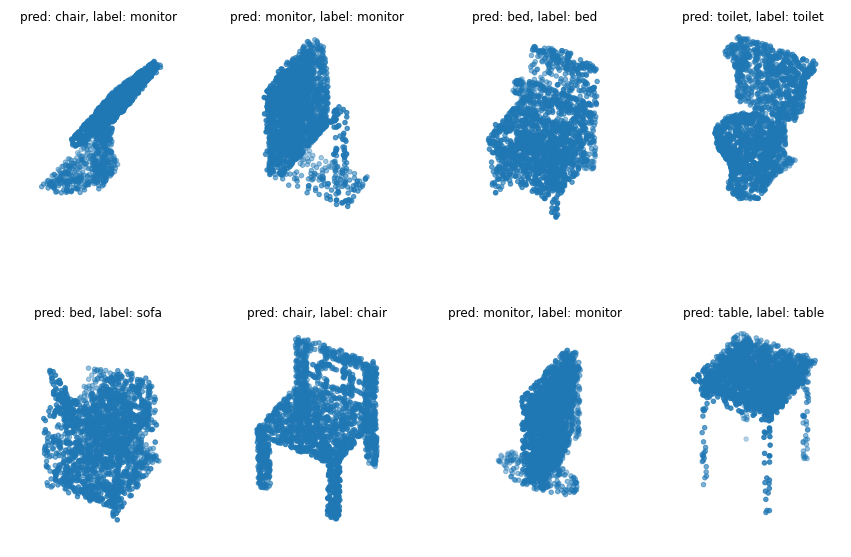
\includegraphics{2.png}

Вывод при обучении:

\begin{Shaded}
\begin{Highlighting}[]
\NormalTok{Epoch }\DecValTok{1}\OperatorTok{/}\DecValTok{20}
\DecValTok{125}\OperatorTok{/}\DecValTok{125} \OperatorTok{[==============================]} \OperatorTok{{-}} \DecValTok{492}\BuiltInTok{s} \DecValTok{4}\BuiltInTok{s}\OperatorTok{/}\NormalTok{step }\OperatorTok{{-}}\NormalTok{ loss}\OperatorTok{:} \FloatTok{3.5283} \OperatorTok{{-}}\NormalTok{ sparse\_categorical\_accuracy}\OperatorTok{:} \FloatTok{0.2902} \OperatorTok{{-}}\NormalTok{ val\_loss}\OperatorTok{:} \FloatTok{210954740446527488.0000} \OperatorTok{{-}}\NormalTok{ val\_sparse\_categorical\_accuracy}\OperatorTok{:} \FloatTok{0.2313}
\NormalTok{Epoch }\DecValTok{2}\OperatorTok{/}\DecValTok{20}
\DecValTok{125}\OperatorTok{/}\DecValTok{125} \OperatorTok{[==============================]} \OperatorTok{{-}} \DecValTok{484}\BuiltInTok{s} \DecValTok{4}\BuiltInTok{s}\OperatorTok{/}\NormalTok{step }\OperatorTok{{-}}\NormalTok{ loss}\OperatorTok{:} \FloatTok{3.0721} \OperatorTok{{-}}\NormalTok{ sparse\_categorical\_accuracy}\OperatorTok{:} \FloatTok{0.3698} \OperatorTok{{-}}\NormalTok{ val\_loss}\OperatorTok{:} \FloatTok{33479804795748352.0000} \OperatorTok{{-}}\NormalTok{ val\_sparse\_categorical\_accuracy}\OperatorTok{:} \FloatTok{0.2985}
\NormalTok{Epoch }\DecValTok{3}\OperatorTok{/}\DecValTok{20}
\DecValTok{125}\OperatorTok{/}\DecValTok{125} \OperatorTok{[==============================]} \OperatorTok{{-}} \DecValTok{491}\BuiltInTok{s} \DecValTok{4}\BuiltInTok{s}\OperatorTok{/}\NormalTok{step }\OperatorTok{{-}}\NormalTok{ loss}\OperatorTok{:} \FloatTok{2.9749} \OperatorTok{{-}}\NormalTok{ sparse\_categorical\_accuracy}\OperatorTok{:} \FloatTok{0.4174} \OperatorTok{{-}}\NormalTok{ val\_loss}\OperatorTok{:} \FloatTok{875655449280512.0000} \OperatorTok{{-}}\NormalTok{ val\_sparse\_categorical\_accuracy}\OperatorTok{:} \FloatTok{0.4306}
\NormalTok{Epoch }\DecValTok{4}\OperatorTok{/}\DecValTok{20}
\DecValTok{125}\OperatorTok{/}\DecValTok{125} \OperatorTok{[==============================]} \OperatorTok{{-}} \DecValTok{486}\BuiltInTok{s} \DecValTok{4}\BuiltInTok{s}\OperatorTok{/}\NormalTok{step }\OperatorTok{{-}}\NormalTok{ loss}\OperatorTok{:} \FloatTok{2.6991} \OperatorTok{{-}}\NormalTok{ sparse\_categorical\_accuracy}\OperatorTok{:} \FloatTok{0.5009} \OperatorTok{{-}}\NormalTok{ val\_loss}\OperatorTok{:} \FloatTok{180347.5469} \OperatorTok{{-}}\NormalTok{ val\_sparse\_categorical\_accuracy}\OperatorTok{:} \FloatTok{0.3282}
\NormalTok{Epoch }\DecValTok{5}\OperatorTok{/}\DecValTok{20}
\DecValTok{125}\OperatorTok{/}\DecValTok{125} \OperatorTok{[==============================]} \OperatorTok{{-}} \DecValTok{486}\BuiltInTok{s} \DecValTok{4}\BuiltInTok{s}\OperatorTok{/}\NormalTok{step }\OperatorTok{{-}}\NormalTok{ loss}\OperatorTok{:} \FloatTok{2.5644} \OperatorTok{{-}}\NormalTok{ sparse\_categorical\_accuracy}\OperatorTok{:} \FloatTok{0.5440} \OperatorTok{{-}}\NormalTok{ val\_loss}\OperatorTok{:} \FloatTok{106151293541679104.0000} \OperatorTok{{-}}\NormalTok{ val\_sparse\_categorical\_accuracy}\OperatorTok{:} \FloatTok{0.4251}
\NormalTok{Epoch }\DecValTok{6}\OperatorTok{/}\DecValTok{20}
\DecValTok{125}\OperatorTok{/}\DecValTok{125} \OperatorTok{[==============================]} \OperatorTok{{-}} \DecValTok{486}\BuiltInTok{s} \DecValTok{4}\BuiltInTok{s}\OperatorTok{/}\NormalTok{step }\OperatorTok{{-}}\NormalTok{ loss}\OperatorTok{:} \FloatTok{2.4421} \OperatorTok{{-}}\NormalTok{ sparse\_categorical\_accuracy}\OperatorTok{:} \FloatTok{0.5755} \OperatorTok{{-}}\NormalTok{ val\_loss}\OperatorTok{:} \FloatTok{424143.7500} \OperatorTok{{-}}\NormalTok{ val\_sparse\_categorical\_accuracy}\OperatorTok{:} \FloatTok{0.4857}
\NormalTok{Epoch }\DecValTok{7}\OperatorTok{/}\DecValTok{20}
\DecValTok{125}\OperatorTok{/}\DecValTok{125} \OperatorTok{[==============================]} \OperatorTok{{-}} \DecValTok{485}\BuiltInTok{s} \DecValTok{4}\BuiltInTok{s}\OperatorTok{/}\NormalTok{step }\OperatorTok{{-}}\NormalTok{ loss}\OperatorTok{:} \FloatTok{2.3482} \OperatorTok{{-}}\NormalTok{ sparse\_categorical\_accuracy}\OperatorTok{:} \FloatTok{0.6021} \OperatorTok{{-}}\NormalTok{ val\_loss}\OperatorTok{:} \FloatTok{9424011788288.0000} \OperatorTok{{-}}\NormalTok{ val\_sparse\_categorical\_accuracy}\OperatorTok{:} \FloatTok{0.5980}
\NormalTok{Epoch }\DecValTok{8}\OperatorTok{/}\DecValTok{20}
\DecValTok{125}\OperatorTok{/}\DecValTok{125} \OperatorTok{[==============================]} \OperatorTok{{-}} \DecValTok{487}\BuiltInTok{s} \DecValTok{4}\BuiltInTok{s}\OperatorTok{/}\NormalTok{step }\OperatorTok{{-}}\NormalTok{ loss}\OperatorTok{:} \FloatTok{2.2929} \OperatorTok{{-}}\NormalTok{ sparse\_categorical\_accuracy}\OperatorTok{:} \FloatTok{0.6221} \OperatorTok{{-}}\NormalTok{ val\_loss}\OperatorTok{:} \FloatTok{523065917440.0000} \OperatorTok{{-}}\NormalTok{ val\_sparse\_categorical\_accuracy}\OperatorTok{:} \FloatTok{0.5991}
\NormalTok{Epoch }\DecValTok{9}\OperatorTok{/}\DecValTok{20}
\DecValTok{125}\OperatorTok{/}\DecValTok{125} \OperatorTok{[==============================]} \OperatorTok{{-}} \DecValTok{489}\BuiltInTok{s} \DecValTok{4}\BuiltInTok{s}\OperatorTok{/}\NormalTok{step }\OperatorTok{{-}}\NormalTok{ loss}\OperatorTok{:} \FloatTok{2.1982} \OperatorTok{{-}}\NormalTok{ sparse\_categorical\_accuracy}\OperatorTok{:} \FloatTok{0.6595} \OperatorTok{{-}}\NormalTok{ val\_loss}\OperatorTok{:} \FloatTok{79335302103040.0000} \OperatorTok{{-}}\NormalTok{ val\_sparse\_categorical\_accuracy}\OperatorTok{:} \FloatTok{0.7236}
\NormalTok{Epoch }\DecValTok{10}\OperatorTok{/}\DecValTok{20}
\DecValTok{125}\OperatorTok{/}\DecValTok{125} \OperatorTok{[==============================]} \OperatorTok{{-}} \DecValTok{492}\BuiltInTok{s} \DecValTok{4}\BuiltInTok{s}\OperatorTok{/}\NormalTok{step }\OperatorTok{{-}}\NormalTok{ loss}\OperatorTok{:} \FloatTok{2.0412} \OperatorTok{{-}}\NormalTok{ sparse\_categorical\_accuracy}\OperatorTok{:} \FloatTok{0.7114} \OperatorTok{{-}}\NormalTok{ val\_loss}\OperatorTok{:} \FloatTok{32762660864.0000} \OperatorTok{{-}}\NormalTok{ val\_sparse\_categorical\_accuracy}\OperatorTok{:} \FloatTok{0.5859}
\NormalTok{Epoch }\DecValTok{11}\OperatorTok{/}\DecValTok{20}
\DecValTok{125}\OperatorTok{/}\DecValTok{125} \OperatorTok{[==============================]} \OperatorTok{{-}} \DecValTok{494}\BuiltInTok{s} \DecValTok{4}\BuiltInTok{s}\OperatorTok{/}\NormalTok{step }\OperatorTok{{-}}\NormalTok{ loss}\OperatorTok{:} \FloatTok{2.0109} \OperatorTok{{-}}\NormalTok{ sparse\_categorical\_accuracy}\OperatorTok{:} \FloatTok{0.7098} \OperatorTok{{-}}\NormalTok{ val\_loss}\OperatorTok{:} \FloatTok{57038135296.0000} \OperatorTok{{-}}\NormalTok{ val\_sparse\_categorical\_accuracy}\OperatorTok{:} \FloatTok{0.6597}
\NormalTok{Epoch }\DecValTok{12}\OperatorTok{/}\DecValTok{20}
\DecValTok{125}\OperatorTok{/}\DecValTok{125} \OperatorTok{[==============================]} \OperatorTok{{-}} \DecValTok{490}\BuiltInTok{s} \DecValTok{4}\BuiltInTok{s}\OperatorTok{/}\NormalTok{step }\OperatorTok{{-}}\NormalTok{ loss}\OperatorTok{:} \FloatTok{1.9475} \OperatorTok{{-}}\NormalTok{ sparse\_categorical\_accuracy}\OperatorTok{:} \FloatTok{0.7417} \OperatorTok{{-}}\NormalTok{ val\_loss}\OperatorTok{:} \FloatTok{6202808329727337562112.0000} \OperatorTok{{-}}\NormalTok{ val\_sparse\_categorical\_accuracy}\OperatorTok{:} \FloatTok{0.5154}
\NormalTok{Epoch }\DecValTok{13}\OperatorTok{/}\DecValTok{20}
\DecValTok{125}\OperatorTok{/}\DecValTok{125} \OperatorTok{[==============================]} \OperatorTok{{-}} \DecValTok{493}\BuiltInTok{s} \DecValTok{4}\BuiltInTok{s}\OperatorTok{/}\NormalTok{step }\OperatorTok{{-}}\NormalTok{ loss}\OperatorTok{:} \FloatTok{2.0223} \OperatorTok{{-}}\NormalTok{ sparse\_categorical\_accuracy}\OperatorTok{:} \FloatTok{0.7234} \OperatorTok{{-}}\NormalTok{ val\_loss}\OperatorTok{:} \FloatTok{5557061689540608.0000} \OperatorTok{{-}}\NormalTok{ val\_sparse\_categorical\_accuracy}\OperatorTok{:} \FloatTok{0.7852}
\NormalTok{Epoch }\DecValTok{14}\OperatorTok{/}\DecValTok{20}
\DecValTok{125}\OperatorTok{/}\DecValTok{125} \OperatorTok{[==============================]} \OperatorTok{{-}} \DecValTok{494}\BuiltInTok{s} \DecValTok{4}\BuiltInTok{s}\OperatorTok{/}\NormalTok{step }\OperatorTok{{-}}\NormalTok{ loss}\OperatorTok{:} \FloatTok{1.9383} \OperatorTok{{-}}\NormalTok{ sparse\_categorical\_accuracy}\OperatorTok{:} \FloatTok{0.7374} \OperatorTok{{-}}\NormalTok{ val\_loss}\OperatorTok{:} \FloatTok{149.8369} \OperatorTok{{-}}\NormalTok{ val\_sparse\_categorical\_accuracy}\OperatorTok{:} \FloatTok{0.5892}
\NormalTok{Epoch }\DecValTok{15}\OperatorTok{/}\DecValTok{20}
\DecValTok{125}\OperatorTok{/}\DecValTok{125} \OperatorTok{[==============================]} \OperatorTok{{-}} \DecValTok{492}\BuiltInTok{s} \DecValTok{4}\BuiltInTok{s}\OperatorTok{/}\NormalTok{step }\OperatorTok{{-}}\NormalTok{ loss}\OperatorTok{:} \FloatTok{1.8217} \OperatorTok{{-}}\NormalTok{ sparse\_categorical\_accuracy}\OperatorTok{:} \FloatTok{0.7675} \OperatorTok{{-}}\NormalTok{ val\_loss}\OperatorTok{:} \FloatTok{2.4758} \OperatorTok{{-}}\NormalTok{ val\_sparse\_categorical\_accuracy}\OperatorTok{:} \FloatTok{0.5088}
\NormalTok{Epoch }\DecValTok{16}\OperatorTok{/}\DecValTok{20}
\DecValTok{125}\OperatorTok{/}\DecValTok{125} \OperatorTok{[==============================]} \OperatorTok{{-}} \DecValTok{506}\BuiltInTok{s} \DecValTok{4}\BuiltInTok{s}\OperatorTok{/}\NormalTok{step }\OperatorTok{{-}}\NormalTok{ loss}\OperatorTok{:} \FloatTok{1.7787} \OperatorTok{{-}}\NormalTok{ sparse\_categorical\_accuracy}\OperatorTok{:} \FloatTok{0.7760} \OperatorTok{{-}}\NormalTok{ val\_loss}\OperatorTok{:} \FloatTok{2338560.7500} \OperatorTok{{-}}\NormalTok{ val\_sparse\_categorical\_accuracy}\OperatorTok{:} \FloatTok{0.7192}
\NormalTok{Epoch }\DecValTok{17}\OperatorTok{/}\DecValTok{20}
\DecValTok{125}\OperatorTok{/}\DecValTok{125} \OperatorTok{[==============================]} \OperatorTok{{-}} \DecValTok{510}\BuiltInTok{s} \DecValTok{4}\BuiltInTok{s}\OperatorTok{/}\NormalTok{step }\OperatorTok{{-}}\NormalTok{ loss}\OperatorTok{:} \FloatTok{1.7970} \OperatorTok{{-}}\NormalTok{ sparse\_categorical\_accuracy}\OperatorTok{:} \FloatTok{0.7853} \OperatorTok{{-}}\NormalTok{ val\_loss}\OperatorTok{:} \FloatTok{146297877168128.0000} \OperatorTok{{-}}\NormalTok{ val\_sparse\_categorical\_accuracy}\OperatorTok{:} \FloatTok{0.6278}
\NormalTok{Epoch }\DecValTok{18}\OperatorTok{/}\DecValTok{20}
\DecValTok{125}\OperatorTok{/}\DecValTok{125} \OperatorTok{[==============================]} \OperatorTok{{-}} \DecValTok{518}\BuiltInTok{s} \DecValTok{4}\BuiltInTok{s}\OperatorTok{/}\NormalTok{step }\OperatorTok{{-}}\NormalTok{ loss}\OperatorTok{:} \FloatTok{1.7527} \OperatorTok{{-}}\NormalTok{ sparse\_categorical\_accuracy}\OperatorTok{:} \FloatTok{0.7870} \OperatorTok{{-}}\NormalTok{ val\_loss}\OperatorTok{:} \FloatTok{6409579659264.0000} \OperatorTok{{-}}\NormalTok{ val\_sparse\_categorical\_accuracy}\OperatorTok{:} \FloatTok{0.6718}
\NormalTok{Epoch }\DecValTok{19}\OperatorTok{/}\DecValTok{20}
\DecValTok{125}\OperatorTok{/}\DecValTok{125} \OperatorTok{[==============================]} \OperatorTok{{-}} \DecValTok{509}\BuiltInTok{s} \DecValTok{4}\BuiltInTok{s}\OperatorTok{/}\NormalTok{step }\OperatorTok{{-}}\NormalTok{ loss}\OperatorTok{:} \FloatTok{1.6873} \OperatorTok{{-}}\NormalTok{ sparse\_categorical\_accuracy}\OperatorTok{:} \FloatTok{0.8066} \OperatorTok{{-}}\NormalTok{ val\_loss}\OperatorTok{:} \FloatTok{62779597095174144.0000} \OperatorTok{{-}}\NormalTok{ val\_sparse\_categorical\_accuracy}\OperatorTok{:} \FloatTok{0.8128}
\NormalTok{Epoch }\DecValTok{20}\OperatorTok{/}\DecValTok{20}
\DecValTok{125}\OperatorTok{/}\DecValTok{125} \OperatorTok{[==============================]} \OperatorTok{{-}} \DecValTok{514}\BuiltInTok{s} \DecValTok{4}\BuiltInTok{s}\OperatorTok{/}\NormalTok{step }\OperatorTok{{-}}\NormalTok{ loss}\OperatorTok{:} \FloatTok{1.6595} \OperatorTok{{-}}\NormalTok{ sparse\_categorical\_accuracy}\OperatorTok{:} \FloatTok{0.8083} \OperatorTok{{-}}\NormalTok{ val\_loss}\OperatorTok{:} \FloatTok{1481432192.0000} \OperatorTok{{-}}\NormalTok{ val\_sparse\_categorical\_accuracy}\OperatorTok{:} \FloatTok{0.6894}
\end{Highlighting}
\end{Shaded}

Исходный код:

\begin{Shaded}
\begin{Highlighting}[]
\CommentTok{"""}
\CommentTok{\# Point cloud classification with PointNet}

\CommentTok{**Author:** [David Griffiths](https://dgriffiths3.github.io)\textless{}br\textgreater{}}
\CommentTok{**Date created:** 2020/05/25\textless{}br\textgreater{}}
\CommentTok{**Last modified:** 2020/05/26\textless{}br\textgreater{}}
\CommentTok{**Description:** Implementation of PointNet for ModelNet10 classification.}

\CommentTok{\# Point cloud classification}

\CommentTok{\#\# Introduction}

\CommentTok{Classification, detection and segmentation of unordered 3D point sets i.e. point clouds}
\CommentTok{is a core problem in computer vision. This example implements the seminal point cloud}
\CommentTok{deep learning paper [PointNet (Qi et al., 2017)](https://arxiv.org/abs/1612.00593). For a}
\CommentTok{detailed intoduction on PointNet see [this blog}
\CommentTok{post](https://medium.com/@luis\_gonzales/an{-}in{-}depth{-}look{-}at{-}pointnet{-}111d7efdaa1a).}

\CommentTok{\#\# Setup}

\CommentTok{If using colab first install trimesh with \textasciigrave{}!pip install trimesh\textasciigrave{}.}
\CommentTok{"""}

\ImportTok{import}\NormalTok{ os}
\ImportTok{import}\NormalTok{ glob}
\ImportTok{import}\NormalTok{ trimesh}
\ImportTok{import}\NormalTok{ numpy }\ImportTok{as}\NormalTok{ np}
\ImportTok{import}\NormalTok{ tensorflow }\ImportTok{as}\NormalTok{ tf}
\ImportTok{from}\NormalTok{ tensorflow }\ImportTok{import}\NormalTok{ keras}
\ImportTok{from}\NormalTok{ tensorflow.keras }\ImportTok{import}\NormalTok{ layers}
\ImportTok{from}\NormalTok{ matplotlib }\ImportTok{import}\NormalTok{ pyplot }\ImportTok{as}\NormalTok{ plt}

\NormalTok{tf.random.set\_seed(}\DecValTok{1234}\NormalTok{)}

\CommentTok{"""\#\# Load dataset}

\CommentTok{We use the ModelNet10 model dataset, the smaller 10 class version of the ModelNet40}
\CommentTok{dataset. First download the data:}

\CommentTok{"""}

\NormalTok{DATA\_DIR }\OperatorTok{=}\NormalTok{ tf.keras.utils.get\_file(}
    \StringTok{"modelnet.zip"}\NormalTok{,}
    \StringTok{"http://3dvision.princeton.edu/projects/2014/3DShapeNets/ModelNet10.zip"}\NormalTok{,}
\NormalTok{    extract}\OperatorTok{=}\VariableTok{True}\NormalTok{,}
\NormalTok{)}
\NormalTok{DATA\_DIR }\OperatorTok{=}\NormalTok{ os.path.join(os.path.dirname(DATA\_DIR), }\StringTok{"ModelNet10"}\NormalTok{)}

\CommentTok{"""We can use the \textasciigrave{}trimesh\textasciigrave{} package to read and visualize the \textasciigrave{}.off\textasciigrave{} mesh files.}

\CommentTok{"""}

\NormalTok{mesh }\OperatorTok{=}\NormalTok{ trimesh.load(os.path.join(DATA\_DIR, }\StringTok{"chair/train/chair\_0001.off"}\NormalTok{))}
\NormalTok{mesh.show()}

\CommentTok{"""To convert a mesh file to a point cloud we first need to sample points on the mesh}
\CommentTok{surface. \textasciigrave{}.sample()\textasciigrave{} performs a unifrom random sampling. Here we sample at 2048 locations}
\CommentTok{and visualize in \textasciigrave{}matplotlib\textasciigrave{}.}

\CommentTok{"""}

\NormalTok{points }\OperatorTok{=}\NormalTok{ mesh.sample(}\DecValTok{2048}\NormalTok{)}

\NormalTok{fig }\OperatorTok{=}\NormalTok{ plt.figure(figsize}\OperatorTok{=}\NormalTok{(}\DecValTok{5}\NormalTok{, }\DecValTok{5}\NormalTok{))}
\NormalTok{ax }\OperatorTok{=}\NormalTok{ fig.add\_subplot(}\DecValTok{111}\NormalTok{, projection}\OperatorTok{=}\StringTok{"3d"}\NormalTok{)}
\NormalTok{ax.scatter(points[:, }\DecValTok{0}\NormalTok{], points[:, }\DecValTok{1}\NormalTok{], points[:, }\DecValTok{2}\NormalTok{])}
\NormalTok{ax.set\_axis\_off()}
\NormalTok{plt.show()}

\CommentTok{"""To generate a \textasciigrave{}tf.data.Dataset()\textasciigrave{} we need to first parse through the ModelNet data}
\CommentTok{folders. Each mesh is loaded and sampled into a point cloud before being added to a}
\CommentTok{standard python list and converted to a \textasciigrave{}numpy\textasciigrave{} array. We also store the current}
\CommentTok{enumerate index value as the object label and use a dictionary to recall this later.}

\CommentTok{"""}

\KeywordTok{def}\NormalTok{ parse\_dataset(num\_points}\OperatorTok{=}\DecValTok{2048}\NormalTok{):}

\NormalTok{    train\_points }\OperatorTok{=}\NormalTok{ []}
\NormalTok{    train\_labels }\OperatorTok{=}\NormalTok{ []}
\NormalTok{    test\_points }\OperatorTok{=}\NormalTok{ []}
\NormalTok{    test\_labels }\OperatorTok{=}\NormalTok{ []}
\NormalTok{    class\_map }\OperatorTok{=}\NormalTok{ \{\}}
\NormalTok{    folders }\OperatorTok{=}\NormalTok{ glob.glob(os.path.join(DATA\_DIR, }\StringTok{"[!README]*"}\NormalTok{))}

    \ControlFlowTok{for}\NormalTok{ i, folder }\KeywordTok{in} \BuiltInTok{enumerate}\NormalTok{(folders):}
        \BuiltInTok{print}\NormalTok{(}\StringTok{"processing class: }\SpecialCharTok{\{\}}\StringTok{"}\NormalTok{.}\BuiltInTok{format}\NormalTok{(os.path.basename(folder)))}
        \CommentTok{\# store folder name with ID so we can retrieve later}
\NormalTok{        class\_map[i] }\OperatorTok{=}\NormalTok{ folder.split(}\StringTok{"/"}\NormalTok{)[}\OperatorTok{{-}}\DecValTok{1}\NormalTok{]}
        \CommentTok{\# gather all files}
\NormalTok{        train\_files }\OperatorTok{=}\NormalTok{ glob.glob(os.path.join(folder, }\StringTok{"train/*"}\NormalTok{))}
\NormalTok{        test\_files }\OperatorTok{=}\NormalTok{ glob.glob(os.path.join(folder, }\StringTok{"test/*"}\NormalTok{))}

        \ControlFlowTok{for}\NormalTok{ f }\KeywordTok{in}\NormalTok{ train\_files:}
\NormalTok{            train\_points.append(trimesh.load(f).sample(num\_points))}
\NormalTok{            train\_labels.append(i)}

        \ControlFlowTok{for}\NormalTok{ f }\KeywordTok{in}\NormalTok{ test\_files:}
\NormalTok{            test\_points.append(trimesh.load(f).sample(num\_points))}
\NormalTok{            test\_labels.append(i)}

    \ControlFlowTok{return}\NormalTok{ (}
\NormalTok{        np.array(train\_points),}
\NormalTok{        np.array(test\_points),}
\NormalTok{        np.array(train\_labels),}
\NormalTok{        np.array(test\_labels),}
\NormalTok{        class\_map,}
\NormalTok{    )}

\CommentTok{"""Set the number of points to sample and batch size and parse the dataset. This can take}
\CommentTok{\textasciitilde{}5minutes to complete.}

\CommentTok{"""}

\NormalTok{NUM\_POINTS }\OperatorTok{=} \DecValTok{2048}
\NormalTok{NUM\_CLASSES }\OperatorTok{=} \DecValTok{10}
\NormalTok{BATCH\_SIZE }\OperatorTok{=} \DecValTok{32}

\NormalTok{train\_points, test\_points, train\_labels, test\_labels, CLASS\_MAP }\OperatorTok{=}\NormalTok{ parse\_dataset(}
\NormalTok{    NUM\_POINTS}
\NormalTok{)}

\CommentTok{"""Our data can now be read into a \textasciigrave{}tf.data.Dataset()\textasciigrave{} object. We set the shuffle buffer}
\CommentTok{size to the entire size of the dataset as prior to this the data is ordered by class.}
\CommentTok{Data augmentation is important when working with point cloud data. We create a}
\CommentTok{augmentation function to jitter and shuffle the train dataset.}

\CommentTok{"""}

\KeywordTok{def}\NormalTok{ augment(points, label):}
    \CommentTok{\# jitter points}
\NormalTok{    points }\OperatorTok{+=}\NormalTok{ tf.random.uniform(points.shape, }\OperatorTok{{-}}\FloatTok{0.005}\NormalTok{, }\FloatTok{0.005}\NormalTok{, dtype}\OperatorTok{=}\NormalTok{tf.float64)}
    \CommentTok{\# shuffle points}
\NormalTok{    points }\OperatorTok{=}\NormalTok{ tf.random.shuffle(points)}
    \ControlFlowTok{return}\NormalTok{ points, label}


\NormalTok{train\_dataset }\OperatorTok{=}\NormalTok{ tf.data.Dataset.from\_tensor\_slices((train\_points, train\_labels))}
\NormalTok{test\_dataset }\OperatorTok{=}\NormalTok{ tf.data.Dataset.from\_tensor\_slices((test\_points, test\_labels))}

\NormalTok{train\_dataset }\OperatorTok{=}\NormalTok{ train\_dataset.shuffle(}\BuiltInTok{len}\NormalTok{(train\_points)).}\BuiltInTok{map}\NormalTok{(augment).batch(BATCH\_SIZE)}
\NormalTok{test\_dataset }\OperatorTok{=}\NormalTok{ test\_dataset.shuffle(}\BuiltInTok{len}\NormalTok{(test\_points)).batch(BATCH\_SIZE)}

\CommentTok{"""\#\#\# Build a model}

\CommentTok{Each convolution and fully{-}connected layer (with exception for end layers) consits of}
\CommentTok{Convolution / Dense {-}\textgreater{} Batch Normalization {-}\textgreater{} ReLU Activation.}

\CommentTok{"""}

\KeywordTok{def}\NormalTok{ conv\_bn(x, filters):}
\NormalTok{    x }\OperatorTok{=}\NormalTok{ layers.Conv1D(filters, kernel\_size}\OperatorTok{=}\DecValTok{1}\NormalTok{, padding}\OperatorTok{=}\StringTok{"valid"}\NormalTok{)(x)}
\NormalTok{    x }\OperatorTok{=}\NormalTok{ layers.BatchNormalization(momentum}\OperatorTok{=}\FloatTok{0.0}\NormalTok{)(x)}
    \ControlFlowTok{return}\NormalTok{ layers.Activation(}\StringTok{"relu"}\NormalTok{)(x)}


\KeywordTok{def}\NormalTok{ dense\_bn(x, filters):}
\NormalTok{    x }\OperatorTok{=}\NormalTok{ layers.Dense(filters)(x)}
\NormalTok{    x }\OperatorTok{=}\NormalTok{ layers.BatchNormalization(momentum}\OperatorTok{=}\FloatTok{0.0}\NormalTok{)(x)}
    \ControlFlowTok{return}\NormalTok{ layers.Activation(}\StringTok{"relu"}\NormalTok{)(x)}

\CommentTok{"""PointNet consists of two core components. The primary MLP network, and the transformer}
\CommentTok{net (T{-}net). The T{-}net aims to learn an affine transformation matrix by its own mini}
\CommentTok{network. The T{-}net is used twice. The first time to transform the input features (n, 3)}
\CommentTok{into a canonical representation. The second is an affine transformation for alignment in}
\CommentTok{feature space (n, 3). As per the original paper we constrain the transformation to be}
\CommentTok{close to an orthogonal matrix (i.e. ||X*X\^{}T {-} I|| = 0).}

\CommentTok{"""}

\KeywordTok{class}\NormalTok{ OrthogonalRegularizer(keras.regularizers.Regularizer):}
    \KeywordTok{def} \FunctionTok{\_\_init\_\_}\NormalTok{(}\VariableTok{self}\NormalTok{, num\_features, l2reg}\OperatorTok{=}\FloatTok{0.001}\NormalTok{):}
        \VariableTok{self}\NormalTok{.num\_features }\OperatorTok{=}\NormalTok{ num\_features}
        \VariableTok{self}\NormalTok{.l2reg }\OperatorTok{=}\NormalTok{ l2reg}
        \VariableTok{self}\NormalTok{.eye }\OperatorTok{=}\NormalTok{ tf.eye(num\_features)}

    \KeywordTok{def} \FunctionTok{\_\_call\_\_}\NormalTok{(}\VariableTok{self}\NormalTok{, x):}
\NormalTok{        x }\OperatorTok{=}\NormalTok{ tf.reshape(x, (}\OperatorTok{{-}}\DecValTok{1}\NormalTok{, }\VariableTok{self}\NormalTok{.num\_features, }\VariableTok{self}\NormalTok{.num\_features))}
\NormalTok{        xxt }\OperatorTok{=}\NormalTok{ tf.tensordot(x, x, axes}\OperatorTok{=}\NormalTok{(}\DecValTok{2}\NormalTok{, }\DecValTok{2}\NormalTok{))}
\NormalTok{        xxt }\OperatorTok{=}\NormalTok{ tf.reshape(xxt, (}\OperatorTok{{-}}\DecValTok{1}\NormalTok{, }\VariableTok{self}\NormalTok{.num\_features, }\VariableTok{self}\NormalTok{.num\_features))}
        \ControlFlowTok{return}\NormalTok{ tf.reduce\_sum(}\VariableTok{self}\NormalTok{.l2reg }\OperatorTok{*}\NormalTok{ tf.square(xxt }\OperatorTok{{-}} \VariableTok{self}\NormalTok{.eye))}

\CommentTok{""" We can then define a general function to build T{-}net layers.}

\CommentTok{"""}

\KeywordTok{def}\NormalTok{ tnet(inputs, num\_features):}

    \CommentTok{\# Initalise bias as the indentity matrix}
\NormalTok{    bias }\OperatorTok{=}\NormalTok{ keras.initializers.Constant(np.eye(num\_features).flatten())}
\NormalTok{    reg }\OperatorTok{=}\NormalTok{ OrthogonalRegularizer(num\_features)}

\NormalTok{    x }\OperatorTok{=}\NormalTok{ conv\_bn(inputs, }\DecValTok{32}\NormalTok{)}
\NormalTok{    x }\OperatorTok{=}\NormalTok{ conv\_bn(x, }\DecValTok{64}\NormalTok{)}
\NormalTok{    x }\OperatorTok{=}\NormalTok{ conv\_bn(x, }\DecValTok{512}\NormalTok{)}
\NormalTok{    x }\OperatorTok{=}\NormalTok{ layers.GlobalMaxPooling1D()(x)}
\NormalTok{    x }\OperatorTok{=}\NormalTok{ dense\_bn(x, }\DecValTok{256}\NormalTok{)}
\NormalTok{    x }\OperatorTok{=}\NormalTok{ dense\_bn(x, }\DecValTok{128}\NormalTok{)}
\NormalTok{    x }\OperatorTok{=}\NormalTok{ layers.Dense(}
\NormalTok{        num\_features }\OperatorTok{*}\NormalTok{ num\_features,}
\NormalTok{        kernel\_initializer}\OperatorTok{=}\StringTok{"zeros"}\NormalTok{,}
\NormalTok{        bias\_initializer}\OperatorTok{=}\NormalTok{bias,}
\NormalTok{        activity\_regularizer}\OperatorTok{=}\NormalTok{reg,}
\NormalTok{    )(x)}
\NormalTok{    feat\_T }\OperatorTok{=}\NormalTok{ layers.Reshape((num\_features, num\_features))(x)}
    \CommentTok{\# Apply affine transformation to input features}
    \ControlFlowTok{return}\NormalTok{ layers.Dot(axes}\OperatorTok{=}\NormalTok{(}\DecValTok{2}\NormalTok{, }\DecValTok{1}\NormalTok{))([inputs, feat\_T])}

\CommentTok{"""The main network can be then implemented in the same manner where the t{-}net mini models}
\CommentTok{can be dropped in a layers in the graph. Here we replicate the network architecture}
\CommentTok{published in the original paper but with half the number of weights at each layer as we}
\CommentTok{are using the smaller 10 class ModelNet dataset.}

\CommentTok{"""}

\NormalTok{inputs }\OperatorTok{=}\NormalTok{ keras.Input(shape}\OperatorTok{=}\NormalTok{(NUM\_POINTS, }\DecValTok{3}\NormalTok{))}

\NormalTok{x }\OperatorTok{=}\NormalTok{ tnet(inputs, }\DecValTok{3}\NormalTok{)}
\NormalTok{x }\OperatorTok{=}\NormalTok{ conv\_bn(x, }\DecValTok{32}\NormalTok{)}
\NormalTok{x }\OperatorTok{=}\NormalTok{ conv\_bn(x, }\DecValTok{32}\NormalTok{)}
\NormalTok{x }\OperatorTok{=}\NormalTok{ tnet(x, }\DecValTok{32}\NormalTok{)}
\NormalTok{x }\OperatorTok{=}\NormalTok{ conv\_bn(x, }\DecValTok{32}\NormalTok{)}
\NormalTok{x }\OperatorTok{=}\NormalTok{ conv\_bn(x, }\DecValTok{64}\NormalTok{)}
\NormalTok{x }\OperatorTok{=}\NormalTok{ conv\_bn(x, }\DecValTok{512}\NormalTok{)}
\NormalTok{x }\OperatorTok{=}\NormalTok{ layers.GlobalMaxPooling1D()(x)}
\NormalTok{x }\OperatorTok{=}\NormalTok{ dense\_bn(x, }\DecValTok{256}\NormalTok{)}
\NormalTok{x }\OperatorTok{=}\NormalTok{ layers.Dropout(}\FloatTok{0.3}\NormalTok{)(x)}
\NormalTok{x }\OperatorTok{=}\NormalTok{ dense\_bn(x, }\DecValTok{128}\NormalTok{)}
\NormalTok{x }\OperatorTok{=}\NormalTok{ layers.Dropout(}\FloatTok{0.3}\NormalTok{)(x)}

\NormalTok{outputs }\OperatorTok{=}\NormalTok{ layers.Dense(NUM\_CLASSES, activation}\OperatorTok{=}\StringTok{"softmax"}\NormalTok{)(x)}

\NormalTok{model }\OperatorTok{=}\NormalTok{ keras.Model(inputs}\OperatorTok{=}\NormalTok{inputs, outputs}\OperatorTok{=}\NormalTok{outputs, name}\OperatorTok{=}\StringTok{"pointnet"}\NormalTok{)}
\NormalTok{model.summary()}

\CommentTok{"""\#\#\# Train model}

\CommentTok{Once the model is defined it can be trained like any other standard classification model}
\CommentTok{using \textasciigrave{}.compile()\textasciigrave{} and \textasciigrave{}.fit()\textasciigrave{}.}

\CommentTok{"""}

\NormalTok{model.}\BuiltInTok{compile}\NormalTok{(}
\NormalTok{    loss}\OperatorTok{=}\StringTok{"sparse\_categorical\_crossentropy"}\NormalTok{,}
\NormalTok{    optimizer}\OperatorTok{=}\NormalTok{keras.optimizers.Adam(learning\_rate}\OperatorTok{=}\FloatTok{0.001}\NormalTok{),}
\NormalTok{    metrics}\OperatorTok{=}\NormalTok{[}\StringTok{"sparse\_categorical\_accuracy"}\NormalTok{],}
\NormalTok{)}

\NormalTok{model.fit(train\_dataset, epochs}\OperatorTok{=}\DecValTok{20}\NormalTok{, validation\_data}\OperatorTok{=}\NormalTok{test\_dataset)}

\CommentTok{"""\#\# Visualize predictions}

\CommentTok{We can use matplotlib to visualize our trained model performance.}

\CommentTok{"""}

\NormalTok{data }\OperatorTok{=}\NormalTok{ test\_dataset.take(}\DecValTok{1}\NormalTok{)}

\NormalTok{points, labels }\OperatorTok{=} \BuiltInTok{list}\NormalTok{(data)[}\DecValTok{0}\NormalTok{]}
\NormalTok{points }\OperatorTok{=}\NormalTok{ points[:}\DecValTok{8}\NormalTok{, ...]}
\NormalTok{labels }\OperatorTok{=}\NormalTok{ labels[:}\DecValTok{8}\NormalTok{, ...]}

\CommentTok{\# run test data through model}
\NormalTok{preds }\OperatorTok{=}\NormalTok{ model.predict(points)}
\NormalTok{preds }\OperatorTok{=}\NormalTok{ tf.math.argmax(preds, }\OperatorTok{{-}}\DecValTok{1}\NormalTok{)}

\NormalTok{points }\OperatorTok{=}\NormalTok{ points.numpy()}

\CommentTok{\# plot points with predicted class and label}
\NormalTok{fig }\OperatorTok{=}\NormalTok{ plt.figure(figsize}\OperatorTok{=}\NormalTok{(}\DecValTok{15}\NormalTok{, }\DecValTok{10}\NormalTok{))}
\ControlFlowTok{for}\NormalTok{ i }\KeywordTok{in} \BuiltInTok{range}\NormalTok{(}\DecValTok{8}\NormalTok{):}
\NormalTok{    ax }\OperatorTok{=}\NormalTok{ fig.add\_subplot(}\DecValTok{2}\NormalTok{, }\DecValTok{4}\NormalTok{, i }\OperatorTok{+} \DecValTok{1}\NormalTok{, projection}\OperatorTok{=}\StringTok{"3d"}\NormalTok{)}
\NormalTok{    ax.scatter(points[i, :, }\DecValTok{0}\NormalTok{], points[i, :, }\DecValTok{1}\NormalTok{], points[i, :, }\DecValTok{2}\NormalTok{])}
\NormalTok{    ax.set\_title(}
        \StringTok{"pred: }\SpecialCharTok{\{:\}}\StringTok{, label: }\SpecialCharTok{\{:\}}\StringTok{"}\NormalTok{.}\BuiltInTok{format}\NormalTok{(}
\NormalTok{            CLASS\_MAP[preds[i].numpy()], CLASS\_MAP[labels.numpy()[i]]}
\NormalTok{        )}
\end{Highlighting}
\end{Shaded}


\end{document}
